%!TEX root =../mapp-challenge-18-game-book.tex
% ^ leave for LaTeXTools build functionality

\phChapterWorksheet{Cross Product}{Cryptic Puzzle 2}

Impressed with your problem-solving ability, the dockworker suggests you head
to the \mappMobidot{} Dojo at the end of Road \(\tan(87.4094^\circ)\).
There, the \textbf{Dojo Master} agrees to battle you, but only on one condition.
He presents you a scroll with the following clues...

\begin{center}
``Only a trainer that has one of these can possibly become HIPCONAM.''

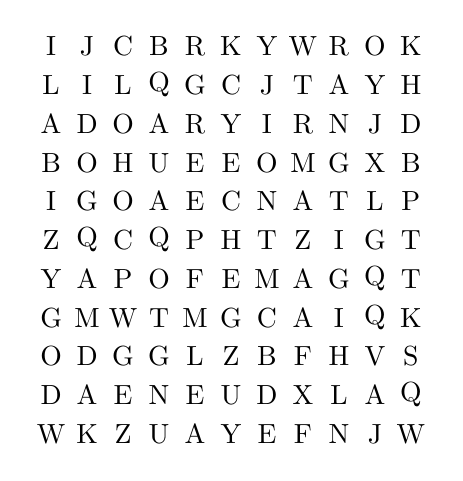
\begin{tikzpicture}[x=1.3em,y=1.4em]
  \node at (0,11) {I};\node at (1,11) {J};\node at (2,11) {C};\node at (3,11) {B};\node at (4,11) {R};\node at (5,11) {K};\node at (6,11) {Y};\node at (7,11) {W};\node at (8,11) {R};\node at (9,11) {O};\node at (10,11) {K};
  \node at (0,10) {L};\node at (1,10) {I};\node at (2,10) {L};\node at (3,10) {Q};\node at (4,10) {G};\node at (5,10) {C};\node at (6,10) {J};\node at (7,10) {T};\node at (8,10) {A};\node at (9,10) {Y};\node at (10,10) {H};
  \node at (0,9) {A};\node at (1,9) {D};\node at (2,9) {O};\node at (3,9) {A};\node at (4,9) {R};\node at (5,9) {Y};\node at (6,9) {I};\node at (7,9) {R};\node at (8,9) {N};\node at (9,9) {J};\node at (10,9) {D};
  \node at (0,8) {B};\node at (1,8) {O};\node at (2,8) {H};\node at (3,8) {U};\node at (4,8) {E};\node at (5,8) {E};\node at (6,8) {O};\node at (7,8) {M};\node at (8,8) {G};\node at (9,8) {X};\node at (10,8) {B};
  \node at (0,7) {I};\node at (1,7) {G};\node at (2,7) {O};\node at (3,7) {A};\node at (4,7) {E};\node at (5,7) {C};\node at (6,7) {N};\node at (7,7) {A};\node at (8,7) {T};\node at (9,7) {L};\node at (10,7) {P};
  \node at (0,6) {Z};\node at (1,6) {Q};\node at (2,6) {C};\node at (3,6) {Q};\node at (4,6) {P};\node at (5,6) {H};\node at (6,6) {T};\node at (7,6) {Z};\node at (8,6) {I};\node at (9,6) {G};\node at (10,6) {T};
  \node at (0,5) {Y};\node at (1,5) {A};\node at (2,5) {P};\node at (3,5) {O};\node at (4,5) {F};\node at (5,5) {E};\node at (6,5) {M};\node at (7,5) {A};\node at (8,5) {G};\node at (9,5) {Q};\node at (10,5) {T};
  \node at (0,4) {G};\node at (1,4) {M};\node at (2,4) {W};\node at (3,4) {T};\node at (4,4) {M};\node at (5,4) {G};\node at (6,4) {C};\node at (7,4) {A};\node at (8,4) {I};\node at (9,4) {Q};\node at (10,4) {K};
  \node at (0,3) {O};\node at (1,3) {D};\node at (2,3) {G};\node at (3,3) {G};\node at (4,3) {L};\node at (5,3) {Z};\node at (6,3) {B};\node at (7,3) {F};\node at (8,3) {H};\node at (9,3) {V};\node at (10,3) {S};
  \node at (0,2) {D};\node at (1,2) {A};\node at (2,2) {E};\node at (3,2) {N};\node at (4,2) {E};\node at (5,2) {U};\node at (6,2) {D};\node at (7,2) {X};\node at (8,2) {L};\node at (9,2) {A};\node at (10,2) {Q};
  \node at (0,1) {W};\node at (1,1) {K};\node at (2,1) {Z};\node at (3,1) {U};\node at (4,1) {A};\node at (5,1) {Y};\node at (6,1) {E};\node at (7,1) {F};\node at (8,1) {N};\node at (9,1) {J};\node at (10,1) {W};

  % \draw (0.5,8.5) rectangle (8.5,9.5);
  % \draw (2.5,6.5) rectangle (3.5,10.5);
  % \draw (7.5,0.5) rectangle (8.5,9.5);
  % \draw (5.5,6.5) rectangle (10.5,7.5);
  % \draw (3.5,3.5) rectangle (8.5,4.5);
  % \draw (3.5,0.5) rectangle (4.5,5.5);
  % \draw (0.5,1.5) rectangle (6.5,2.5);
\end{tikzpicture}

Lightning \(\times\) Plant \hfill
Undead \(\times\) Flame \hfill
Aqua \(\times\) Ordinary \hfill
Flame \(\times\) Magic
\end{center}

A voice belonging to your mentor echoes in your head...
``The key to winning \mappMobidash{} battles is understanding how types match up.''
You know that some \mappMobidot{} types are weak against some types, while
super effective against others. But you're not convinced that's what this scroll
is referring to. Can you \textbf{unscramble} the meaning of the \mappMobidot{} Master's scroll?


% Include below for aucTeX integration
%%% Local Variables:
%%% mode: latex
%%% TeX-master: "../mapp-challenge-18-game-book"
%%% End:
